%%% --- define page size --- %%%
% standard US letter and margins
\documentclass[letterpaper,12pt]{article}
\usepackage[letterpaper, 
            top=2.5cm, 
            bottom=2.5cm, 
            left=3.5cm, 
            right=2.5cm, 
            marginparwidth=2cm
            ]{geometry}

% A4 and margins
% \documentclass[a4paper,12pt]{article}
% \usepackage[a4paper, top=2cm, bottom=2cm, left=2cm, right=2cm, marginparwidth=2cm]{geometry}


%%% --- spacing --- %%%
\usepackage{setspace}
\onehalfspacing
% spacing in figure captions
\usepackage{caption}
\captionsetup{font=small, labelfont=bf, skip=5pt}

%%% --- Language and font encodings --- %%%
\usepackage[english]{babel}
% \usepackage[utf8x]{inputenc}
\usepackage[utf8]{inputenc}
\usepackage{booktabs}
\usepackage{tabu}


%%% --- font style --- %%%
\usepackage{titlesec}
\usepackage[T1]{fontenc}
% \usepackage{helvet}
% \usepackage{tgtermes}
% \usepackage{mathptmx} % times new roman
% \usepackage{helvet} % or helvet
% \renewcommand{\familydefault}{\sfdefault}
% default font
\renewcommand{\familydefault}{\rmdefault}

%%% -- Titles --- %%%
\titleformat{\section}
  % {\normalfont\sffamily\Large\bfseries\color{blue}}
  {\normalfont\rmfamily\Large\bfseries\color{black}}
  {\thesection}{1em}{}
\titleformat{\subsection}
  % {\normalfont\sffamily\large\bfseries\color{cyan}}
  {\normalfont\rmfamily\large\bfseries\color{black}}
  {\thesubsection}{1em}{}

%%% --- Text float around figures --- %%%
%  control how much space appears around floats
\setlength{\floatsep}{12pt plus 2pt minus 2pt}
\setlength{\textfloatsep}{12pt plus 2pt minus 2pt}

%%% --- Figure numbering --- %%%
\usepackage{amsmath}
\numberwithin{figure}{section}
\numberwithin{table}{section}


%%% --- Useful packages --- %%%
\usepackage{subcaption}
\usepackage{graphicx}
\usepackage{float}
\usepackage{svg}
\usepackage{indentfirst}
%\usepackage{apacite}
\usepackage[colorinlistoftodos]{todonotes}
\usepackage[colorlinks=true, allcolors=blue]{hyperref}
\usepackage{multirow}
\usepackage{enumitem}
\setlist{  
  listparindent=\parindent,
  parsep=0pt,
}

% Table
\usepackage{tabularray}
\renewcommand{\arraystretch}{1.2}  % Adjust the line height in tables
\setlength{\tabcolsep}{10pt}  % Adjust the column separation in tables


% citation format: ACS (American Chemical Society) 
\usepackage{achemso}


%% --- REAL PAGE CONTENT STARTS --- %%
\title{\bfseries Research Update}
% \author{Jian Huang \\ Write Your Student ID}
\author{Jian Huang}
\date{2024 Sep}

\begin{document}
\maketitle
\begin{sloppypar}   % avoid new indentations of new paragraphs & overfull warnings
% Project 1
\section{\textbf{Study domain-domain interactions of the CheA using Hyres}}
\subsection{Goal and motivation}
Bacterial chemotaxis enables mobile bacteria to move toward or away from attractants or repellents. The chemotaxis pathways for sensing surrounding chemicals rely on a chemosensory array of so-called core-signaling units (CSUs) \cite{muokEngineeredChemotaxisCore2020}, consisting of transmembrane chemoreceptors, the histidine kinase CheA and an adaptor protein CheW. Many copies of the CSUs can form highly ordered array on the surface of bacterial cell membrane. The chemosensory array can integrate cooperatively the sensory signaling from surrounding chemicals to regulate the autophosphorylation activity of the CheA, which will trigger a series of downstream phosphoration processes (on CheY etc) and eventually modulate the cell's flagella motors \cite{briegelMobilityTwoKinase2013}.

\begin{figure}[H]
    \centering
    \includegraphics[width=400pt]{CSU.png}
    \caption{Core Signaling Units on the E. coli cell membrane surface (The left panel) and the model for the CSU structure. Current understandings of those players are listed below the figure.}
    \label{fig:CSU}
\end{figure}


\subsection{Previously on this project}
\begin{enumerate}
    \item Close inspection of the P1/P1' dimerization interface proposed by Tom revealed that the interface has too many unsaturated negatively charged residues, meaning the proposed interface might not be biophysically feasible.
\end{enumerate}

\subsection{Hyres simulation setup}
    Here, I adopted a lower temperature (380 K) for the CheA Hyres simulation while keeping other restraint setups the same.
\begin{table}[H]
    \small
    \centering
    \caption{Simulation setup and status}
    \begin{tblr}{
      width = \linewidth,
      colspec = {Q[255]Q[95]Q[290]Q[160]Q[135]},
      cell{6}{3} = {fg=red},
      cell{7}{3} = {fg=red},
      cell{8}{3} = {fg=red},
      hline{1-2,9} = {-}{},
    }
    CheA dimer System            & Temp. & Restraints                                                & Time             & Status \\
    "Parallel" P1/P1'     & 350 K       & w P1/P1' restraints                             & 2 us * 6 conf. & Done   \\
    "Parallel" P1/P1'     & 400 K       & w P1/P1' restraints                             & 2 us * 6 conf. & Done   \\
    "Antiparallel" P1/P1' & 350 K       & w P1/P1' restraints                             & 2 us * 6 conf. & Done   \\
    "Antiparallel" P1/P1' & 400 K       & w P1/P1' restraints                             & 2 us * 6 conf. & Done   \\
    "Parallel" P1/P1'    & 350 K       & \textcolor{red}{\textbf{w/o}} P1/P1' restraints & 2 us * 6 conf. &  Done   \\
    "Parallel" P1/P1'     & 400 K       & \textcolor{red}{\textbf{w/o}} P1/P1' restraints & 2 us * 6 conf. &  Done  \\ 
    \textbf{"Parallel" P1/P1'} & \textbf{380 K}  & \textcolor{red}{\textbf{w/o}} P1/P1' restraints & 2 us * 6 conf. & Done \\ 
    \end{tblr}
    \end{table}

\subsection{Distance and contact analysis}
To examine the "\textit{trans-}" productive mode where the P1 from one chain would be phosphorylated by the P4 domain from another chain, I tracked the distances between P1-H48 and ATP in the P4 domains.

\begin{description}[style=nextline,labelindent=0.5cm]
    \item[1. Distance analysis.] I first calculated the distance between P1-H48-C-alpha atom and the P3 atom of the ATP molecule (the ending phosphate group) as a function of simulation time. The measurement directly reflects distance between the substrate and the phosphorylation center, which would represent a "\textbf{productive}" contacting mode.

    \item[2. Contacting frequency analysis.] On the basis of the above distance analysis, I further examine the pairwise contact frequencies between residues on the P1 and P4 domains when P1 and P4 are contacting in the productive mode. I first used a distance cutoff of 20 \AA between P1-H48 and ATP to extract frames where P1 and P4 are productively contacting, and then a contacting cutoff of 15 \AA was used for residue-level pairwise contacts.
\end{description}
\newpage

% Project 2
\section{\textbf{Project Title 2}}

\subsection{Goal and Motivation}
\lipsum[21]

\begin{figure}[H]
    \centering
    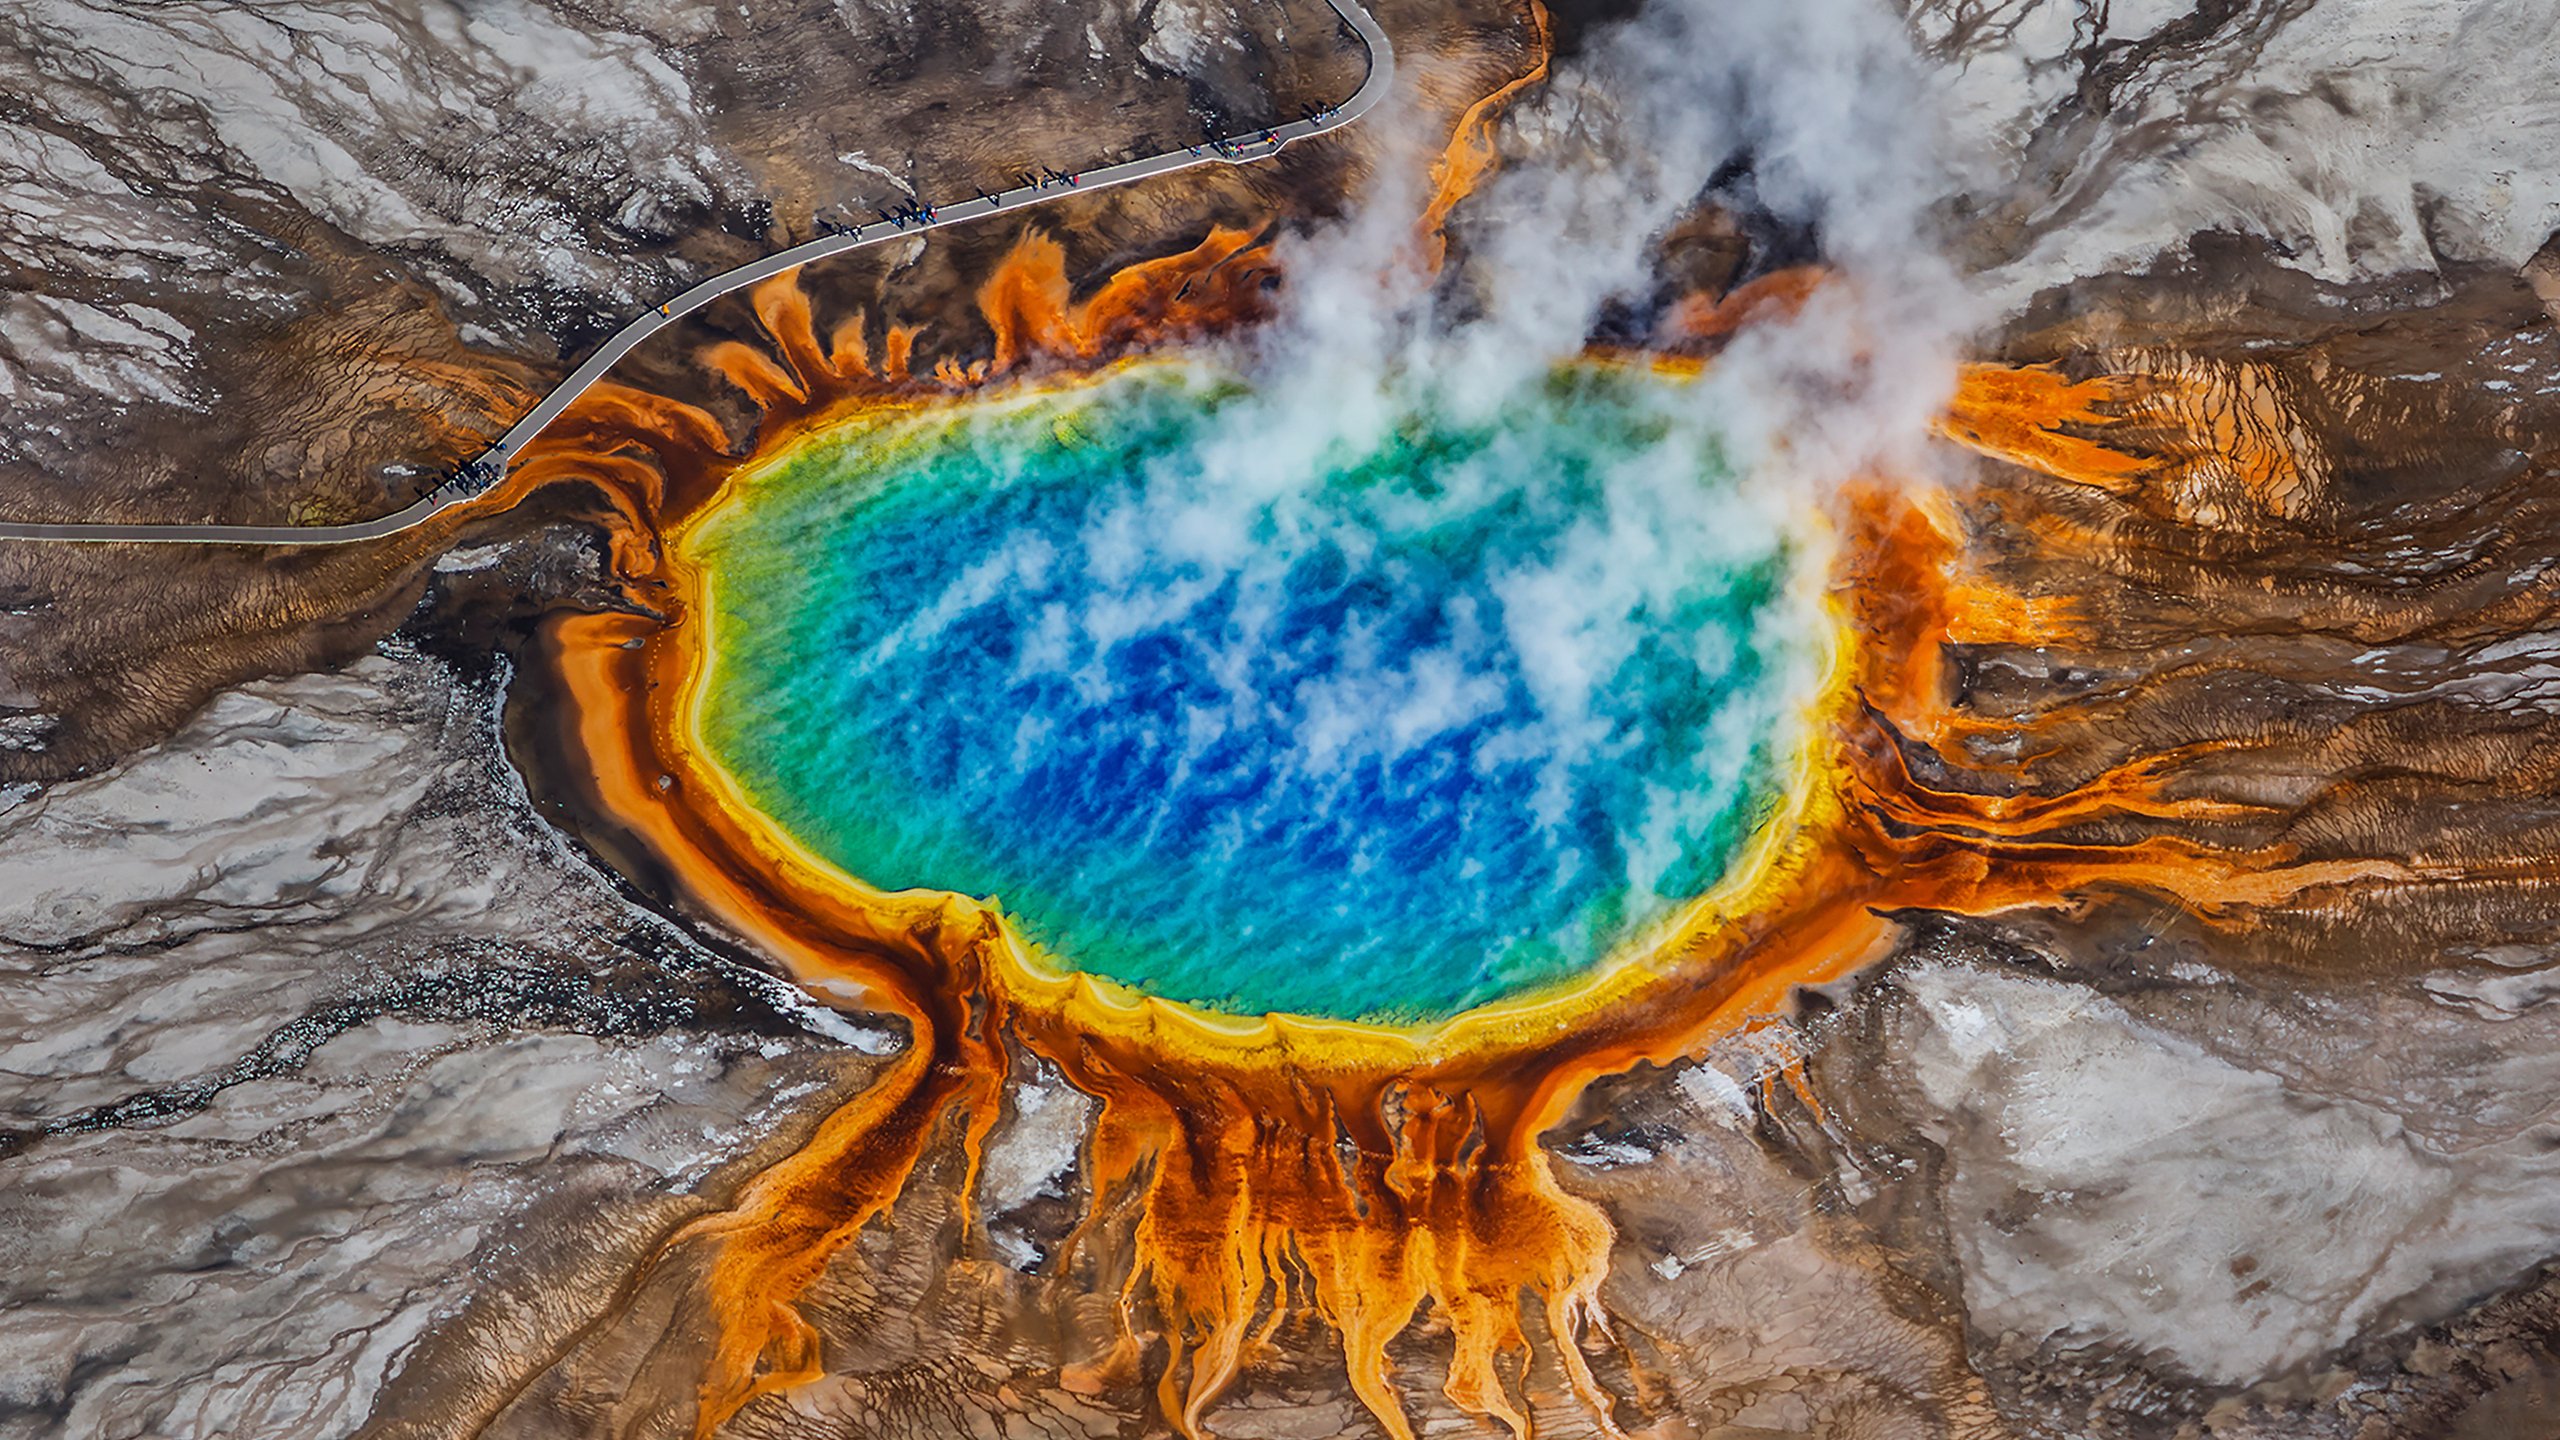
\includegraphics[width=400pt]{assets/figures/YellowstoneSpring.jpg}
    \caption{A placehold for the figure caption}
    \label{fig:label2}
\end{figure}


\subsection{An Example of plotting with Tikz}
\lipsum[28]

\begin{figure}[H]
\centering
\begin{tikzpicture}
    \begin{axis}[
        xlabel={X-axis},
        ylabel={Y-axis},
        title={A Simple Plot}
    ]
    \addplot[color=red,mark=*] coordinates {
        (1,1)
        (2,4)
        (3,9)
        (4,16)
        (5,25)
    };
    \end{axis}
\end{tikzpicture}
\caption{A placehold for the figure caption}
\end{figure}

\lipsum[25]

\newpage

\newpage

% \bibliographystyle{plain}
\bibliography{refs}

\end{sloppypar}
\end{document}